% TikZ redraw for exercise 3-16
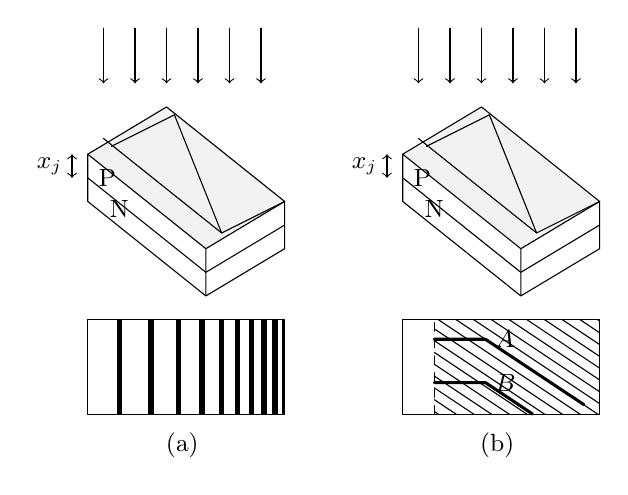
\begin{tikzpicture}[font=\small,line cap=round,line join=round]
\foreach\x/\name in {0/a,4/b}{\begin{scope}[xshift=\x cm]\filldraw[fill=gray!10](0,0)--(1.5,-1.2)--(2.5,-.6)--(1, .6)--cycle;\draw(0,0)--(0,-.6)--(1.5,-1.8)--(2.5,-1.2)--(2.5,-.6) (1.5,-1.2)--(1.5,-1.8);\draw(0,-.3)--(1.5,-1.5)--(2.5,-.9);\draw(.2,.2)--(1.7,-1)--(2.5,-.6);\draw(.3,.1)--(1.1,.5);\draw(1.7,-1)--(1.1,.5);\foreach\a in {.2,.6,1,1.4,1.8,2.2}\draw[->](\a,1.6)--(\a,.9);\node at(.25,-.3){P};\node at(.4,-.7){N};\draw[<->](-.2,0)--node[left]{$x_j$}(-.2,-.3);\node at(1.2,-3.7){(\name)};\end{scope}}
\begin{scope}[yshift=-3.3cm]\draw(0,0)rectangle(2.5,1.2);\clip(0,0)rectangle(2.5,1.2);\foreach\a in {.4,.8,1.15,1.45,1.7,1.9,2.08,2.24,2.38,2.5}\draw[line width=2pt](\a,0)--(\a,1.2);\end{scope}
\begin{scope}[xshift=4cm,yshift=-3.3cm]\draw(0,0)rectangle(2.5,1.2);\begin{scope}\clip(.4,0)rectangle(2.5,1.2);\foreach\y in {-3,-2.85,...,3}\draw(0,\y)--(3,{\y-2});\end{scope}\draw[dashed](.4,0)--(.4,1.2);\draw[line width=1.1pt](.4,.95)--(1.05,.95)--(2.3,.12);\draw[line width=1.1pt](.4,.4)--(1.05,.4)--(1.65,0);\node[right]at(1.05,.95){$A$};\node[right]at(1.05,.4){$B$};\end{scope}
\end{tikzpicture}
